% Things to clean up:
%

% For transparencies add [trans] after document class:
% documentclass[trans]{beamer}
% Basic setup:
% Load the necessary packages:
% Preview environment:
% Title page:

\documentclass[serif,professionalfont,red,aspectratio=169]{beamer}
%%%%%%%%%%%%%%%%%%%%%%%%%%%%%%%%%%%%%%%%%%%%%%%%%%%%%%%%%%%%%%%%%%%%%%%%%%%%%%%%%%%%%%%%%%%%%%%%%%%%%%%%%%%%%%%%%%%%%%%%%%%%%%%%%%%%%%%%%%%%%%%%%%%%%%%%%%%%%%%%%%%%%%%%%%%%%%%%%%%%%%%%%%%%%%%%%%%%%%%%%%%%%%%%%%%%%%%%%%%%%%%%%%%%%%%%%%%%%%%%%%%%%%%%%%%%
\usepackage{xcolor}
\usepackage[english]{babel}
\usepackage[latin1]{inputenc}
\usepackage{times}
\usepackage{amsmath}
\usepackage{amssymb}
\usepackage{graphicx}
\usepackage{tikz}
\usepackage{pgflibrarysnakes}
\usepackage{pgflibraryarrows}
\usepackage[para,online,flushleft]{threeparttable}
\usepackage{verbatim}
\usepackage{ upgreek }
%\usepackage[displaymath,textmath,sections,graphics,floats]{preview}
\usepackage{hyperref}
\usepackage{url}
\setcounter{MaxMatrixCols}{10}
%TCIDATA{OutputFilter=LATEX.DLL}
%TCIDATA{Version=5.50.0.2960}
%TCIDATA{<META NAME="SaveForMode" CONTENT="1">}
%TCIDATA{BibliographyScheme=Manual}
%TCIDATA{LastRevised=Thursday, October 30, 2014 08:58:08}
%TCIDATA{<META NAME="GraphicsSave" CONTENT="32">}

\mode<beamer>
{
\usetheme{Warsaw}
\usecolortheme{lily}
%\setbeamercovered{highly dynamic}
\defbeamertemplate*{footline}{}{}
\setbeamertemplate{navigation symbols}{}
%\setbeamerfont{page number in head/foot}{size=\large}
%\setbeamerfont{footline}{size=\fontsize{9}{11}\selectfont}
\setbeamertemplate{footline}{%
    \raisebox{5pt}{\makebox[\paperwidth]{\hfill\makebox[20pt]{\color{gray}
          \scriptsize\insertframenumber}}}\hspace*{5pt}}
\setbeamertemplate{footline}[frame number]
  }
\mode<trans>
{
\usetheme{default}
\usecolortheme{dove}
\useoutertheme{infolines}
\defbeamertemplate*{footline}{}{}
  }
%\PreviewEnvironment*{frame}
\newtheorem{assumption}{Assumption}
\newtheorem{proposition}{Proposition}
\newtheorem{remark}{Remark}
\subject{Seminar}

%\setbeamertemplate{itemize subitem}[square]
%\setbeamertemplate{itemize subsubitem}[triangle]
\setbeamertemplate{itemize subitem}[triangle]
%Pooja's Modification
\newcommand{\MYhref}[3][blue]{\href{#2}{\color{#1}{#3}}}%
\definecolor{greens}{rgb}{0.0, 0.5, 0.0}
\definecolor{blues}{rgb}{0.0, 0.18, 0.39}
\begin{document}


\title{\textrm{Topic 6:
Economic Growth Facts }}
\author{Prof. Pete Klenow \\ \vspace{3mm} {\small }\textcolor{red}{Klenow@Stanford.edu}}
\date{Econ 52 \\ \vspace{3mm}Fall 2019\\ \vspace{3mm} {\small } Thu 3:30-5:30, Rm. 364}

\begin{frame}
\titlepage
\end{frame}
%%%%%%

\begin{frame}[t]
\frametitle{Topic 6 Contents}
\begin{table}
\centering
    \begin{tabular}{l l l}
    \vspace{4mm}
 Growth Accounting&\hspace{30mm} &6.4 -6.7 
\\ \vspace{4mm}
The Future of U.S. Growth&\hspace{30mm} & 6.8 -6.13
\\ \vspace{4mm}
Development Accounting &\hspace{30mm}&6.14 -6.15 
\\ \vspace{4mm}
Misallocation&\hspace{30mm} & 6.16 -6.26
\\ \vspace{4mm}
Convergence and Divergence&\hspace{30mm}& 6.27 -6.34 
\\ \vspace{4mm}
Globalization and Growth&\hspace{30mm}&6.35 -6.38 
\\\vspace{4mm}
Taxation and Growth&\hspace{30mm}&6.39 -6.40 
\\\vspace{4mm}
Rising inequality&\hspace{30mm}&6.41 -6.47\\
    \end{tabular}
\end{table}
\end{frame}
%%%%%%
\begin{frame}[t]
\frametitle{Old Notation in Topic 6}
\begin{table}
\centering
    \begin{tabular}{l l l}
       \multicolumn{3}{l}{$g_Z=$  growth rate of variable $Z$ }\\
       \\
       \multicolumn{3}{l}{$h=$ human capital per worker}\\
   \\
      $Y$ = real GDP  &   $N$ = hours worked  &   $K$ = physical capital  \\
 \\
 A = TFP  &   pop = population &\\
 \\
         \multicolumn{3}{l}{MPK (MPN) = marginal product of capital (labor)} \\
    \end{tabular}
\end{table}
\end{frame}
%%%%%%
\begin{frame}[t]
\frametitle{Growth Accounting}
\end{frame}
%%%%%%
\begin{frame}[t]
\frametitle{U.S. Growth Accounting}
\begin{table}
\centering
{\renewcommand{\arraystretch}{1.2}
    \begin{tabular}{c c c c c}
    \cline{3-5}
      && \multicolumn{3}{c}{Contribution form }\\
      Period & Output per hour &$K/Y$ & Labor Composition & Labor-Aug.TFP\\
     \hline
     \textbf{1948-2013} & \textbf{2.5} &\textbf{0.1} &\textbf{0.3} &\textbf{2.0}\\
     1948-1973&3.3 &-0.2 &0.3 &3.2\\
     1973-1990 & 1.6 &0.5 &0.3 &0.8\\
     1990-1995 &1.6 &0.2 &0.7 &0.7\\
     1995-2000 &3.0 &0.3 &0.3&2.3\\
     2000-2007&2.7 &0.2 &0.3 &2.2\\
     2007-2013&1.7 &0.1 &0.5 &1.1\\
    \end{tabular}}
\end{table}
\small{Note: Average annual growth rates in present) for output per hour and its components for the private business sector, following equation (3). Source: authors calculations using bureau of Labor statistics, Multifactor Productivity Trends, August 21, 2014.} 
\end{frame}
%%%%%%
\begin{frame}[t]
\frametitle{Jones growth accounting for the U.S.}
\begin{align*}
    \textcolor{blues}{y^\ast\approx \left(\dfrac{K}{Y}\right)^\beta \cdot h\cdot (R\&D \ intensity)^\gamma \cdot L^\gamma}
\end{align*}
\begin{table}
\centering
    \begin{tabular}{c c c c c}
    & \textcolor{greens}{Solow} & \textcolor{greens}{Lucas} & \textcolor{greens}{Romer/AH/GH} & \textcolor{greens}{J/K/S}\\
    2.0& 0.0 & 0.4 & 1.2 & 0.4\\
    (100\%)& (0\%)& (20\%)&(58\%)&(21\%)
    \end{tabular}
\end{table}
\end{frame}
%%%%%%
\begin{frame}[t]
\frametitle{TFP Growth Differences}
\begin{center}
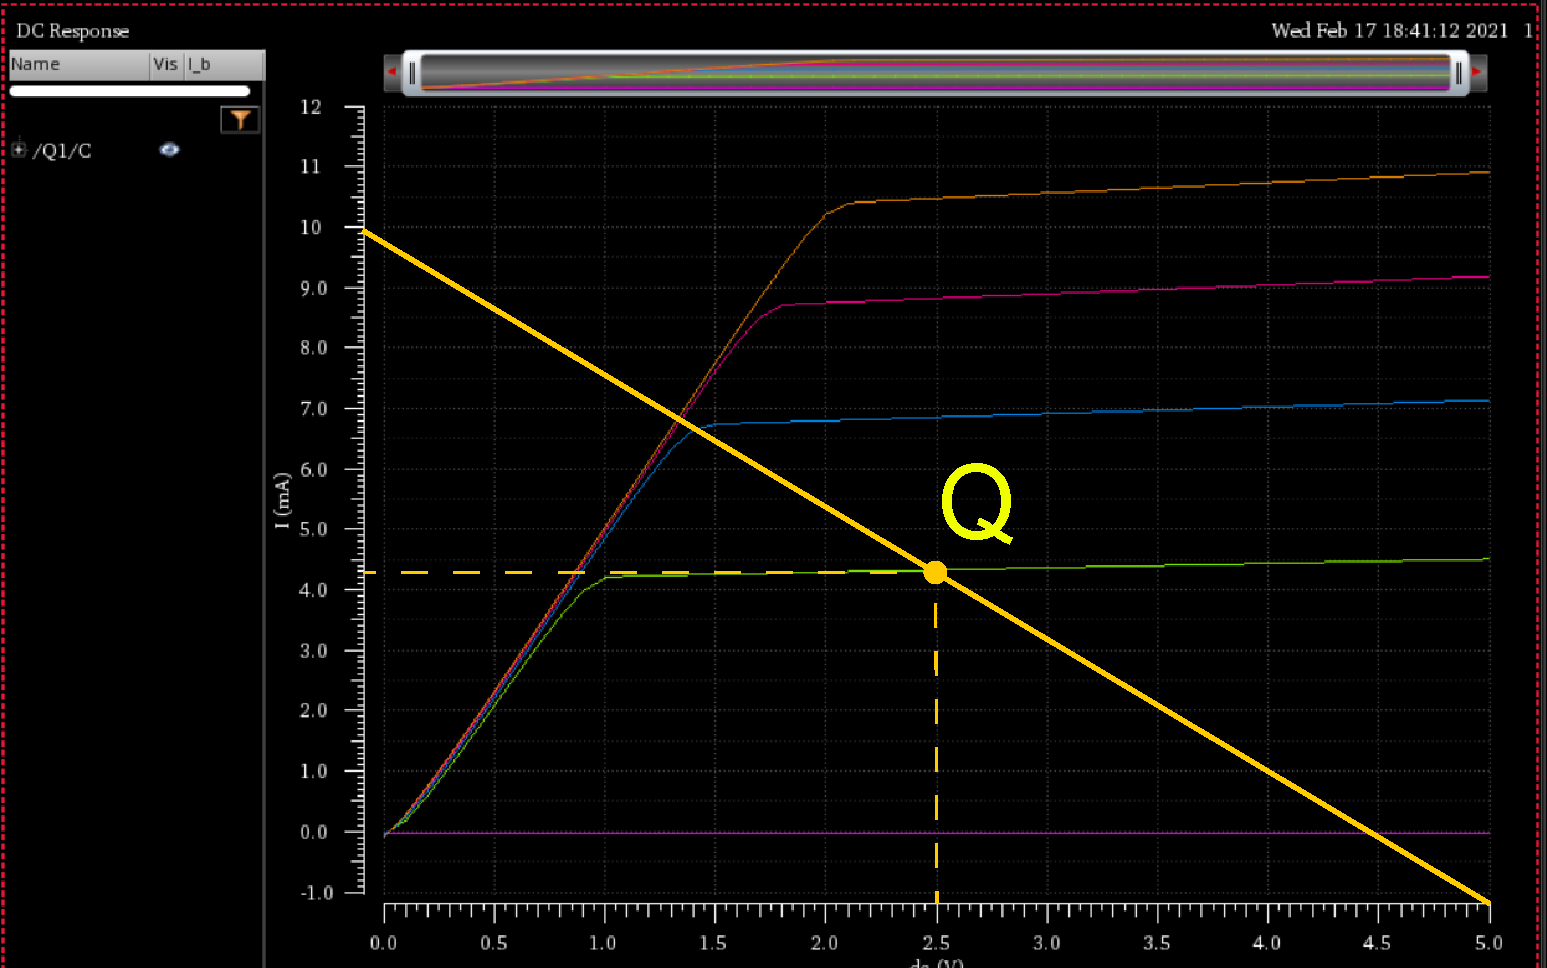
\includegraphics[width=0.3\textwidth]{Images/1.png}
\end{center}
\end{frame}

%%%%%%
\begin{frame}[t]
\frametitle{U.S. TFP growth slowdown}
\begin{center}
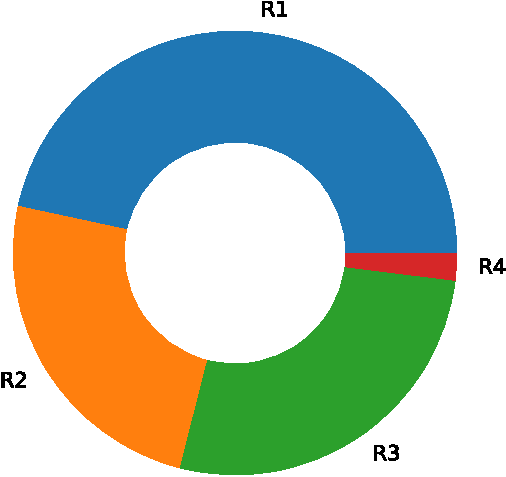
\includegraphics[width=0.7\textwidth]{Images/2.png}
\end{center}
\end{frame}

%%%%%%
\begin{frame}[t]
\frametitle{The Future of U.S. growth}
\vspace{2mm}
\begin{itemize}
\item Reasons for pessimism 
\vspace{2mm}
\begin{itemize}
\item Business dynamism has declined
\vspace{2mm}
\item Educational attainment is leveling off 
\vspace{2mm}
\item \textcolor{blues}{Population growth has fallen} 
\vspace{2mm}
\item \textcolor{blues}{H-1B visas have become more restrictive} 
\vspace{2mm}
\item \textcolor{blues}{Baumol's Cost Disease}
\vspace{4mm}
\end{itemize}
\item Reasons for optimism 
\vspace{2mm}
\begin{itemize}
\item China and India (each as populous as US+EU+Japan) 
\vspace{2mm}
\item How many future Curies and Edisons await everywhere? 
\vspace{2mm}
\item Robots, AI and "The Singularity"
\end{itemize}
\end{itemize}
\end{frame}
%%%%%%
%%%%%%
\begin{frame}[t]
\frametitle{}
\begin{center}
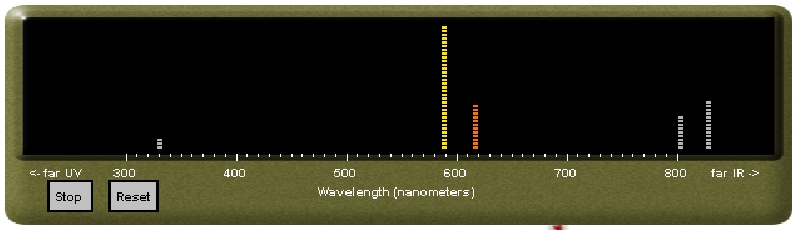
\includegraphics[width=0.55\textwidth]{Images/3.png}
\end{center}
\end{frame}
%%%%%%
%%%%%%
\begin{frame}[t]
\frametitle{}
\begin{center}
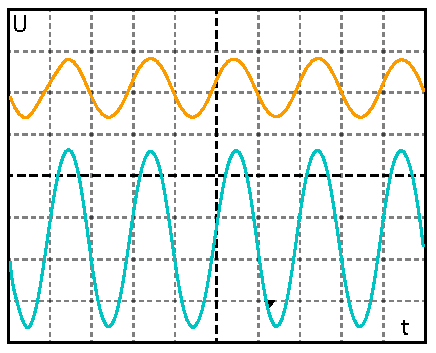
\includegraphics[width=0.8\textwidth]{Images/4.png}
\end{center}
\end{frame}
%%%%%%
\begin{frame}[t]
\frametitle{}
\begin{center}
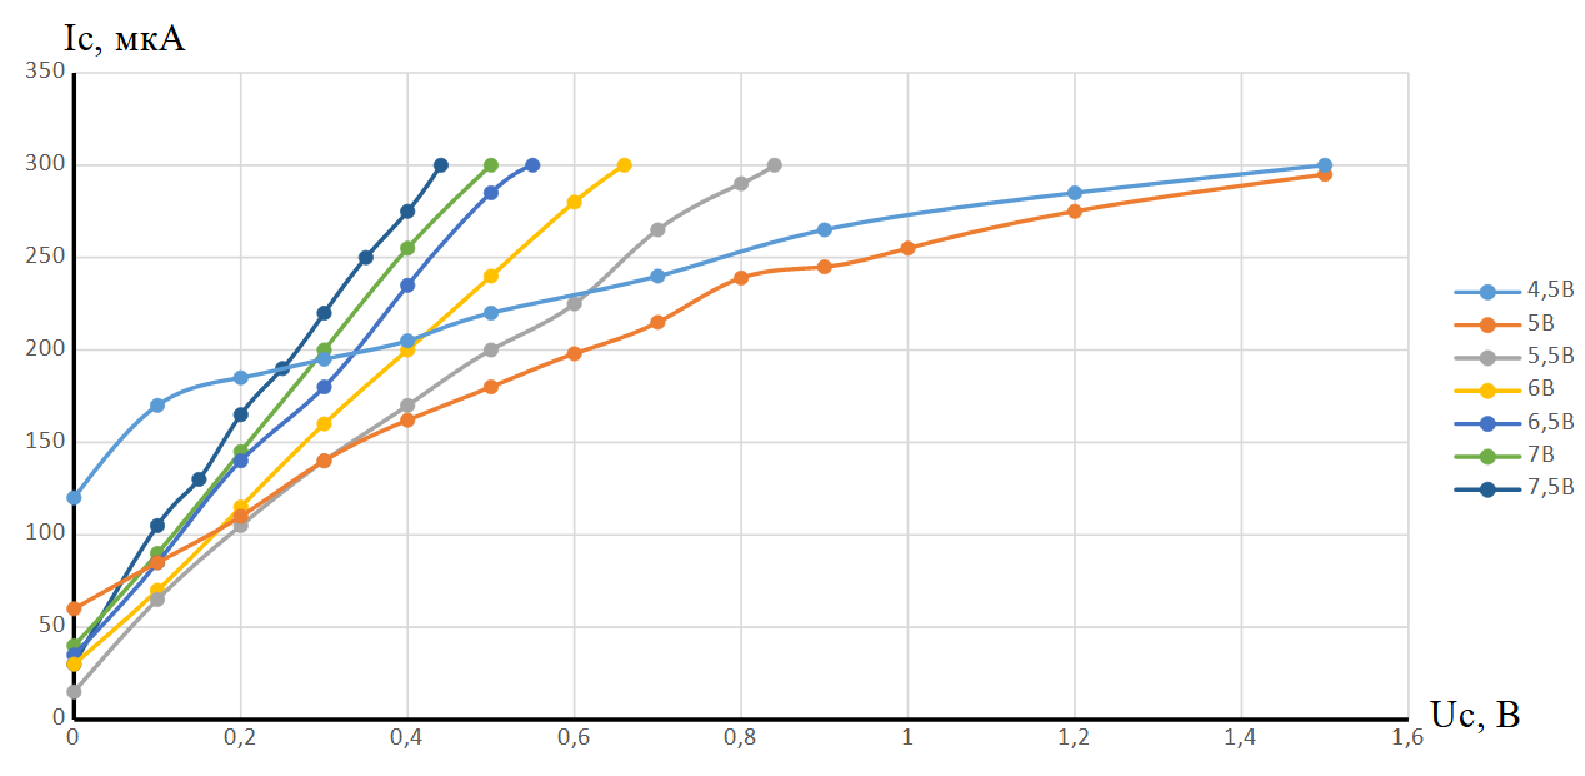
\includegraphics[width=0.8\textwidth]{Images/5.png}
\end{center}
\end{frame}
%%%%%%
\begin{frame}[t]
\frametitle{Notes on the Future of U.S. growth}
\vspace{2mm}
\begin{itemize}
\item Declining business dynamism since around 1980
\vspace{2mm}
\begin{itemize}
\item falling rates of firm entry
\vspace{2mm}
\item falling \% of employment at young firms
\vspace{2mm}
\item falling rates of job reallocation (creation + destruction)
\vspace{2mm}
\item growing barriers to entry from monopoly power?
\end{itemize}
\vspace{4mm}
\item Baumol's Cost Disease
\begin{itemize}
\vspace{2mm}
\item Rising spending share on low TFP growth sectors
\end{itemize}
\vspace{4mm}
\item Rising research intensity in China and India (BIG countries)
\begin{itemize}
\vspace{2mm}
\item More generally, lots of untapped talent all over the world
\end{itemize}
\end{itemize}
\end{frame}
%%%%%%
\begin{frame}[t]
\frametitle{Development Accounting}
\vspace{4mm}
For country $j$  vs. the U.S. in a given year : 
\vspace{2mm}
\begin{align*}
    \dfrac{Y_j/N_j}{Y_{US}/N_{US}}=\bigg\lgroup \dfrac{A_j}{A_{US}}\bigg\rgroup^{\frac{1}{1-\alpha}}%
    \bigg\lgroup \dfrac{K_j/Y_j}{K_{US}/Y_{US}}\bigg\rgroup^{\frac{1}{1-\alpha}}
\end{align*}
\end{frame}
%%%%%%
\begin{frame}[t]
\frametitle{2017 PPP GDP per worker, $\sim$100 countries
}
\vspace{4mm}
Average difference from U.S. Y/N explained by:
\begin{table}
\centering
\renewcommand*\arraystretch{1.3}
    \begin{tabular}{l l}
    \textcolor{red}{K/Y}&5\%\\ 
    \textcolor{red}{A}&95\%\\
    \end{tabular}
\end{table}
\vspace{4mm}
Attempts to further break down the 95\% from A:
\begin{table}
\centering
\renewcommand*\arraystretch{1.3}
    \begin{tabular}{l l}
    \textcolor{red}{Human Capital per worker}&40\%\\
\textcolor{red}{Technology, misallocation}&50\%\\
    \end{tabular}
\end{table}
\end{frame}
%%%%%%
\begin{frame}[t]
\frametitle{Three Main Sources of TFP Differences}
\vspace{4mm}
Human capital per worker 

\vspace{2mm}
\hspace{8mm}Quantity of education
\vspace{2mm}

\hspace{8mm}Quality of education 
\vspace{2mm}

\hspace{8mm}Skills learned on the job 

\vspace{2mm}
\hspace{8mm}Health

\vspace{8mm}

Technology (distance to the WTF)

\vspace{8mm}

Allocative efficiency
\end{frame}
%%%%%%
\begin{frame}[t]
\frametitle{}
\begin{center}
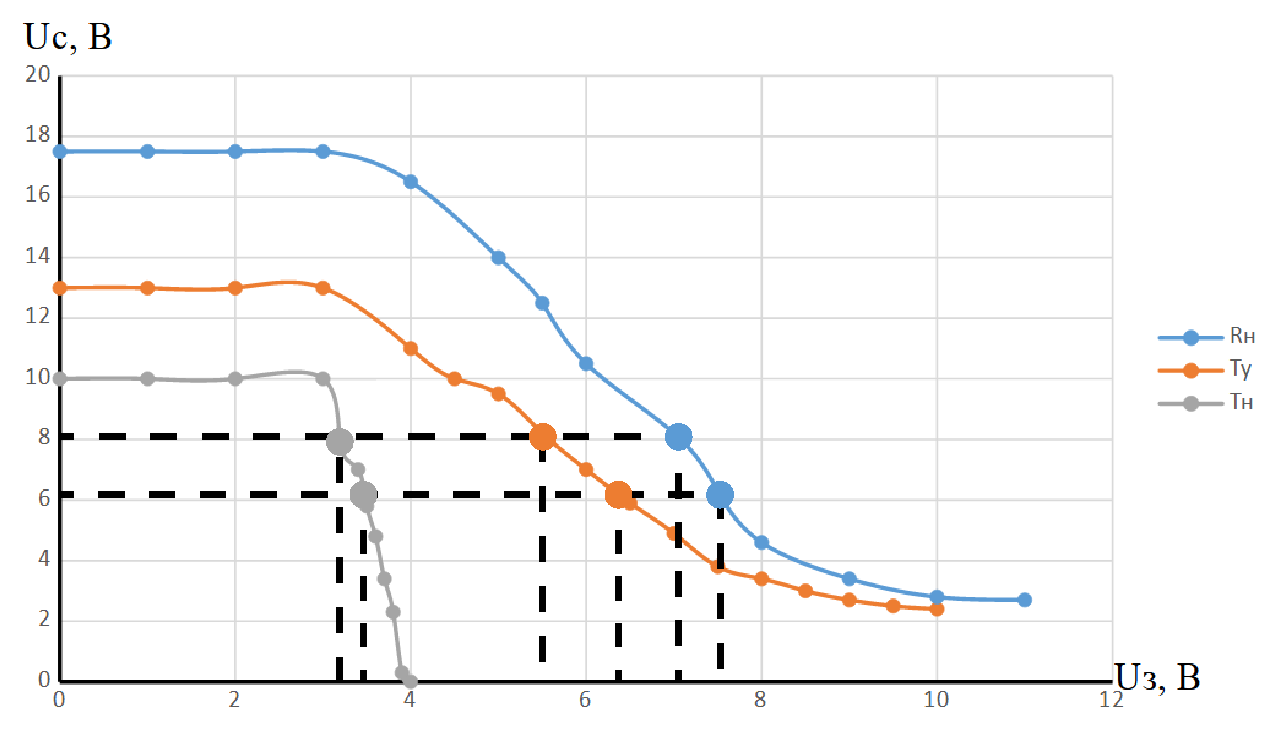
\includegraphics[width=0.8\textwidth]{Images/6.png}
\end{center}
\end{frame}
%%%%%%
\begin{frame}[t]
\frametitle{Misallocation and TFP
}
\vspace{4mm}
Efficient allocation: $MPK_j=MPK_i, MPN_j=MPN_i$ across all firms $i, j$  in an economy.
\vspace{8mm}

Misallocation: $MPK_j \neq MPK_i$ or $MPN_j \neq MPN_i$ across all firms $i, j$  in an economy.
\vspace{8mm}

If misallocation exists, then reallocating a unit of K, N from low to high MPK, MPN increases TFP
\end{frame}
%%%%%%
\begin{frame}[t]
\frametitle{Misallocation and TFP Derivation}
\end{frame}
%%%%%%
\begin{frame}[t]
\frametitle{Dispersion of MPK and MPN within Mfg}
\vspace{2mm}
Rank firms by their MPK (or MPN), then calculate the ratio of (say) the $90^{th}$ percentile firm's MPK to the $10^{th}$ percentile firm's MPK.
\begin{table}
\centering
\renewcommand*\arraystretch{1.8}
    \begin{tabular}{l l l l}
   & \underline{U.S.} & \underline{India} & \underline{China}\\
   $90^{th}/10^{th}$ percentiles & 2.4 & 6.7 &4.9\\
   $75^{th}/25^{th}$ percentiles & 1.3 & 2.5&2.3\\
    \end{tabular}
\end{table}
\vspace{4mm}
\textcolor{red}{Looks like more misallocation in China, India than in the U.S.}\\
\vspace{4mm}
\small{Source:  Hsieh and Klenow} (2009)
\end{frame}
%%%%%%
\begin{frame}[t]
\frametitle{Potential Sources of Misallocation}
\vspace{4mm}
Regulation of entry
\vspace{4mm}

Regulation of labor
\vspace{4mm}

Monopolies
\vspace{4mm}

State-owned enterprises
\vspace{4mm}

State-owned banks
\vspace{4mm}

Trade barriers
\vspace{4mm}

Restrictions on FDI
\end{frame}
%%%%%%
\begin{frame}[t]
\frametitle{}
\begin{center}
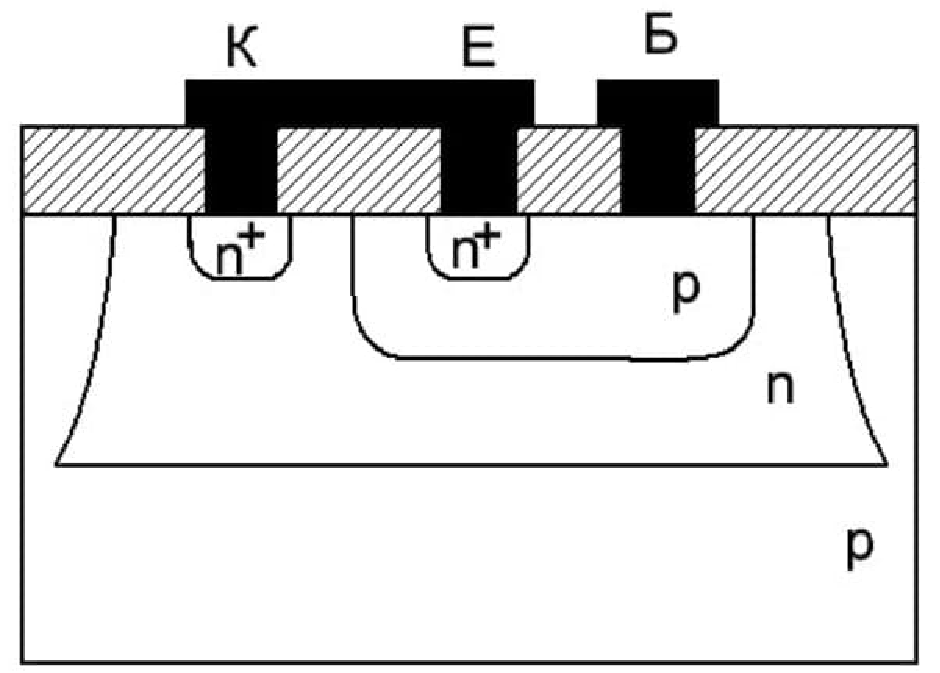
\includegraphics[width=0.5\textwidth]{Images/7.png}
\end{center}
\end{frame}
%%%%%%
\begin{frame}[t]
\frametitle{}
\begin{center}
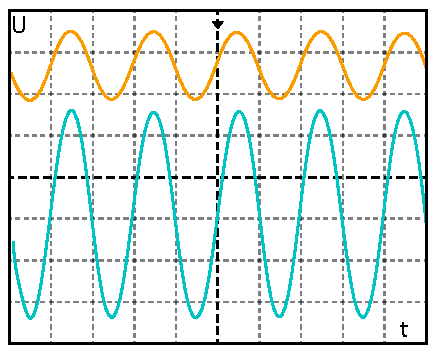
\includegraphics[width=0.55\textwidth]{Images/8.png}
\end{center}
\end{frame}
%%%%%%%%%%%%%%%%%%%%%%%%%%%%%%
\begin{frame}[t]
\frametitle{Evidence on sources of misallocation} 
For each country, the \textcolor{red}{World Bank} estimates the cost of:
\begin{itemize}
\vspace{2mm}
\item Starting a business
\vspace{1mm}
\item Obtaining a construction permit 
\vspace{1mm}
\item Getting electricity
\vspace{1mm}
\item Registering property
\vspace{1mm}
\item  Getting credit
\vspace{1mm}
\item Protecting minority investors
\vspace{1mm}
\item Paying taxes
\vspace{1mm}
\item Trading across borders
\vspace{1mm}
\item Enforcing contracts
\vspace{1mm}
\item Resolving insolvency
\vspace{1mm}
\item Employing workers
\end{itemize}
\vspace{2mm}
Source: DoingBusiness.org
\end{frame}
%%%%%%
\begin{frame}[t]
\frametitle{Firm Growth After Entry}
\begin{center}
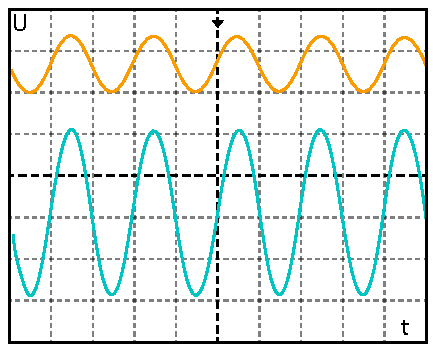
\includegraphics[width=0.5\textwidth]{Images/9.png}
\end{center}
\small{Source: Hsieh and Klenow (2014)}
\end{frame}
%%%%%%%%%%%%%%%%%%%%%%%%%%%%%%
\begin{frame}[t]
\frametitle{Falling misallocation of talent}
\begin{center}
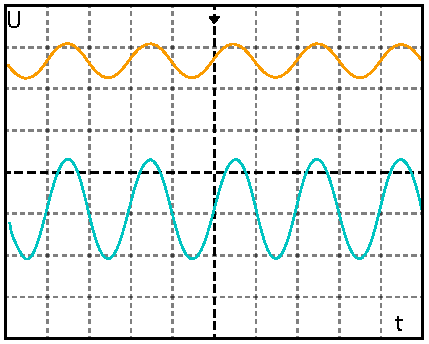
\includegraphics[width=0.6\textwidth]{Images/10.png}
\end{center}
\small{Source: Hsieh, Hurst, Jones and Klenow (2019)}
\end{frame}
%%%%%%%%%%%%%%%%%%%%%%%%%%%%%%
%%%%%%
\begin{frame}[t]
\frametitle{Convergence and Divergence}
\vspace{2mm}
\textcolor{red}{Convergence} =  \textit{\textcolor{blue}{falling}} differences in log (Y/pop) across countries.\\ 
\vspace{4mm}
\underline{Episodes of convergence:} 
\vspace{2mm}
\begin{enumerate}
\item East vs. West since 1950.
\item U.S. states 1880-1980. 
\item Rich nations 1950-1990.
\end{enumerate}
\vspace{4mm}
\textcolor{red}{Divergence} =  \textit{\textcolor{blue}{rising}} differences in GDP per capita.
\vspace{4mm}

\underline{Episodes of divergence} 
\vspace{2mm}
\begin{enumerate}
\item East vs. West from 1800 to 1950. 
\item 100+ countries 1960-2000, when countries weighted equally.\\ 
\textbf{But not if countries are weighted by population given China, India.}
\end{enumerate}
\end{frame}
%%%%%%
%%%%%%
\begin{frame}[t]
\frametitle{}
\begin{center}
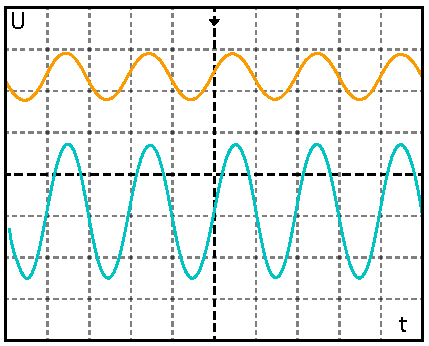
\includegraphics[width=0.8\textwidth]{Images/11.png}
\end{center}
\end{frame}
%%%%%%%%%%%%%%%%%%%%%%%%%
\begin{frame}[t]
\frametitle{}
\begin{center}
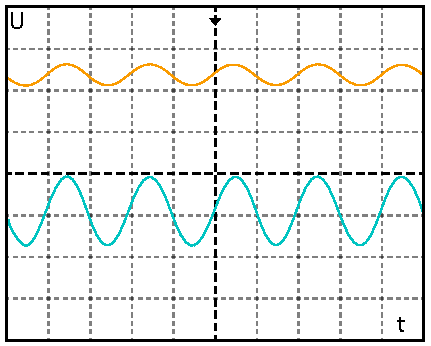
\includegraphics[width=0.58\textwidth]{Images/12.png}
\end{center}
\end{frame}
%%%%%%%%%%%%%%%%%%%%%%%%%
\begin{frame}[t]
\frametitle{}
\begin{center}
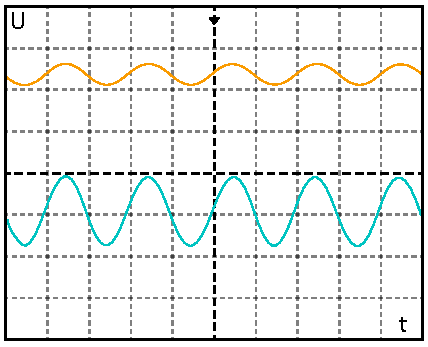
\includegraphics[width=0.55\textwidth]{Images/13.png}
\end{center}
\end{frame}
%%%%%%%%%%%%%%%%%%%%%%%%%
\begin{frame}[t]
\frametitle{}
\begin{center}
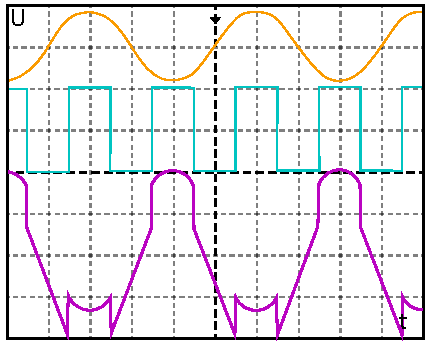
\includegraphics[width=1\textwidth]{Images/14.png}
\end{center}
\end{frame}
%%%%%%%%%%%%%%%%%%%%%%%%%
\begin{frame}[t]
\frametitle{}
\begin{center}
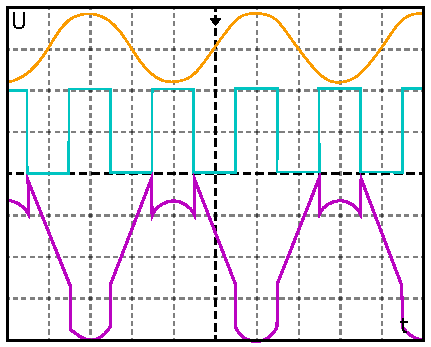
\includegraphics[width=0.8\textwidth]{Images/15.png}
\end{center}
\end{frame}
%%%%%%%%%%%%%%%%%%%%%%%%%
%%%%%%
\begin{frame}[t]
\frametitle{Against Geographic/Cultural Determinism}
\vspace{4mm}
\textcolor{red}{Relative income diverged after policies diverged:}
\vspace{4mm}

\hspace{8mm}West Germany vs. East Germany 1945-1990
\vspace{2mm}

\hspace{8mm}		South Korea vs. North Korea 1955-present
\vspace{2mm}		
		
\hspace{8mm}		Hong Kong vs. China 1960-1978
\vspace{2mm}		
		
\hspace{8mm}		Botswana vs. Zimbabwe 1980-present

\vspace{8mm}		
		
\hspace{8mm}See Acemoglu and Robinson (2012) \textit{Why Nations Fail}.

\vspace{2mm}		
		
\hspace{16mm}Inclusive vs. Extractive institutions.

\vspace{2mm}
\begin{center}
    \MYhref{http://whynationsfail.com/}{WhyNationsFail.com}
\end{center}
\end{frame}
%%%%%%
\begin{frame}[t]
\frametitle{}
\begin{center}
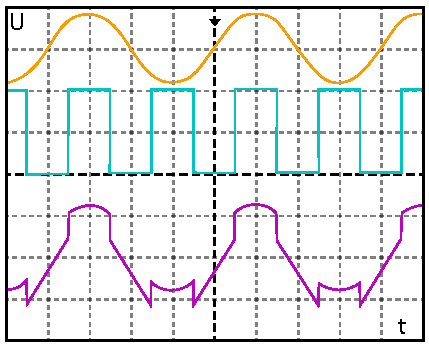
\includegraphics[width=0.8\textwidth]{Images/16.png}
\end{center}
\small{Source: Acemoglu (2009)}
\end{frame}
%%%%%%%%%%%%%%%%%%%%%%%%%
\begin{frame}[t]
\frametitle{Is globalization good for growth?}
\textcolor{greens}{Trade}

\vspace{2mm}
\hspace{8mm}Exploiting comparative advantage increases TFP.
\vspace{2mm}

\hspace{8mm}Competition also promotes higher TFP.

\vspace{2mm}
\hspace{8mm}But increases inequality, hurts some workers/firms.

\vspace{4mm}
\textcolor{greens}{FDI}
\vspace{2mm}

\hspace{8mm}Brings technology, capital, and access to markets.
\vspace{2mm}

\hspace{8mm}Expands the pie, and labor averages 70\% of the gains.
\vspace{2mm}

\hspace{8mm}Foreign firms pay higher wages than domestic firms.
\vspace{4mm}

\textcolor{greens}{Inequality}

\vspace{2mm}
\hspace{8mm}Growing evidence that many low-skilled workers lose.
\end{frame}
%%%%%%%%%%%%%%%%%%%%%%%%%%%
\begin{frame}[t]
\frametitle{}
\begin{center}
\includegraphics[width=0.55\textwidth]{Images/17.png}
\end{center}
\end{frame}
%%%%%%%%%%%%%%%%%%%%%%%%%%%%%%%
\begin{frame}[t]
\frametitle{}
\begin{figure}
\centering
\begin{minipage}{.5\textwidth}
  \centering
  \includegraphics[width=1\textwidth]{Images/18.png}
\end{minipage}%
\begin{minipage}{.5\textwidth}
  \centering
  \includegraphics[width=0.9\textwidth]{Images/19.png}
\end{minipage}
\end{figure}
\end{frame}
%%%%%%%%%%%%%%%%%%%%%%%%%
%%%%%%%%%%%%%%%%%%%%%%%%%%%%%%%
\begin{frame}[t]
\frametitle{}
\begin{center}
\includegraphics[width=0.45\textwidth]{Images/20.png}
\end{center}
\end{frame}
%%%%%%%%%%%%%%%%%%%%%%%%%
\begin{frame}[t]
\frametitle{}
\begin{center}
\includegraphics[width=0.85\textwidth]{Images/21.png}
\end{center}
\end{frame}
%%%%%%%%%%%%%%%%%%%%%%%%%%%%%%%
%%%%%%%%%%%%%%%%%%%%%%%%%%%%%%%
\begin{frame}[t]
\frametitle{Positive correlation between average tax rate and Y/pop}
\textcolor{greens}{Puzzling?
}

\vspace{2mm}
\begin{itemize}
\item[~] Higher tax rate on capital income should decrease K/Y and therefore Y/N.  Impact of tax rate on labor income is 
	more ambiguous
\end{itemize}

\vspace{4mm}
\textcolor{greens}{Causal?
}
\vspace{2mm}
\begin{itemize}
\item[~] Some of the additional revenue is spent on government 	investments such as education, infrastructure, and health.
\end{itemize}
\vspace{4mm}

\textcolor{greens}{Or just reverse causality?
}
\vspace{2mm}
\begin{itemize}
\item[~] Rich countries may choose more redistribution.  And well functioning states may be better able to collect revenue.
\end{itemize}
\end{frame}
%%%%%%%%%%%%%%%%%%%%%%%%%%%%%%%

\begin{frame}[t]
\frametitle{Rising inequality}
\vspace{2mm}
\begin{itemize}
\item Within the U.S. since 1980 or so
\begin{itemize}
\vspace{2mm}
\item Wages
\vspace{2mm}
\item Income
\vspace{2mm}
\item Wealth
\end{itemize}
\vspace{4mm}
\item Within many other countries as well
\begin{itemize}
\vspace{2mm}
\item China and India, for example
\vspace{2mm}
\item But not all countries (France, for example)
\end{itemize}
\vspace{4mm}
\item Suggests a common cause
\begin{itemize}
\vspace{2mm}
\item Leading candidate is the nature of technological change
\end{itemize}
\vspace{4mm}
\item May lower average utility, lead to policies blocking creative destruction
\end{itemize}
\end{frame}
%%%%%%%%%%%%%%%%%%%%%%%%%%%%%%%

%%%%%%%%%%%%%%%%%%%%%%%%%%%%%%%
\begin{frame}[t]
\frametitle{}
\begin{center}
  \begin{figure}
  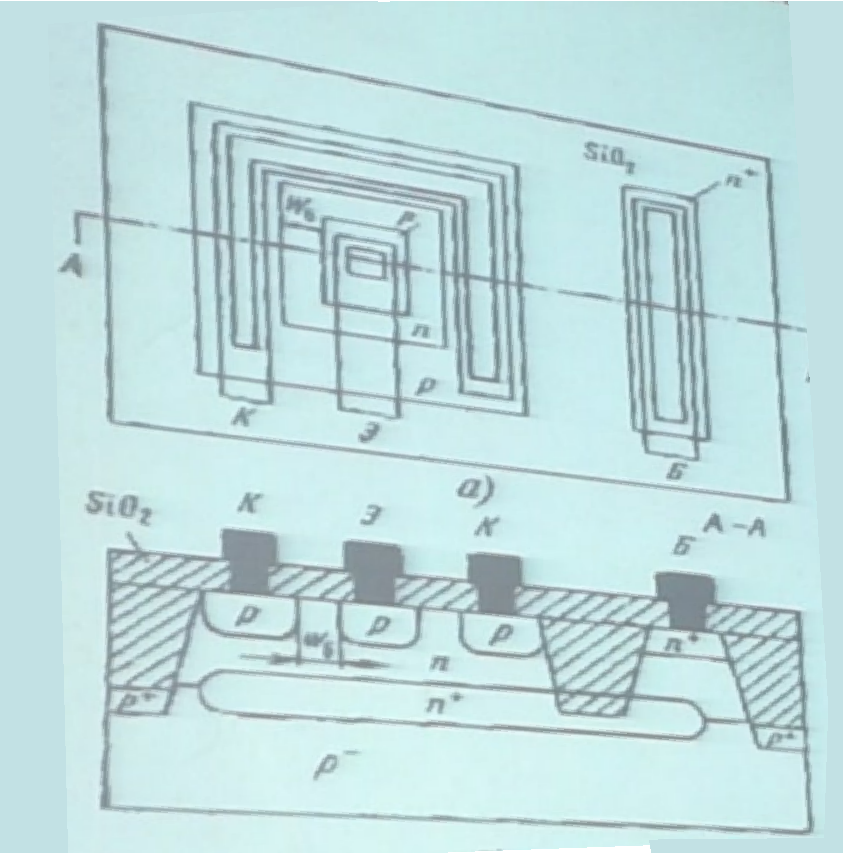
\includegraphics[width=0.55\textwidth]{Images/22.png}
\end{figure} 
\end{center}
\end{frame}
%%%%%%%%%%%%%%%%%%%%%%%%%%%%%%%
\begin{frame}[t]
\frametitle{}
\begin{center}
  \begin{figure}
  \includegraphics[width=0.9\textwidth]{Images/23.png}
\end{figure} 
\end{center}
\end{frame}
%%%%%%%%%%%%%%%%%%%%%%%%%%%%%%%
\begin{frame}[t]
\frametitle{}
\begin{center}
  \begin{figure}
  \includegraphics[width=0.8\textwidth]{Images/24.png}
\end{figure} 
\end{center}
\end{frame}
%%%%%%%%%%%%%%%%%%%%%%%%%%%%%%%
\begin{frame}[t]
\frametitle{}
\begin{center}
  \begin{figure}
  \includegraphics[width=0.8\textwidth]{Images/25.png}
\end{figure} 
\end{center}
\end{frame}
%%%%%%%%%%%%%%%%%%%%%%%%%%%%%%%
\begin{frame}[t]
\frametitle{}
\begin{center}
  \begin{figure}
  \includegraphics[width=0.58\textwidth]{Images/26.png}
\end{figure} 
\end{center}
\end{frame}
%%%%%%%%%%%%%%%%%%%%%%%%%%%%%%%
\begin{frame}[t]
\frametitle{}
\begin{center}
  \begin{figure}
  \includegraphics[width=1\textwidth]{Images/27.png}
\end{figure} 
\end{center}
\end{frame}
%%%%%%%%%%%%%%%%%%%%%%%%%%%%%%%
%%%%%%%%%%%%%%%%%%%%%%
\begin{frame}[t]
\frametitle{Key Points (1/3)}
\vspace{2mm}
Growth Accounting divides growth in Y/L into contributions from
A (TFP) and K/Y.

\vspace{8mm}
Most of growth comes from TFP growth, not K/Y growth. This is
true of the U.S. and other countries.

\vspace{8mm}
TFP growth is faster in many follower countries, but far from all.

\vspace{8mm}
In the U.S., rising human capital is important for TFP growth, but
rising research effort has played an even bigger role.

\vspace{8mm}
Secular stagnation: future U.S. TFP growth may be 1.5\% (faster
than recent 1\%, slower than secular average of 2.0\%)
\end{frame}
%%%%%%%%%%%%%%%%%%%%%%
\begin{frame}[t]
\frametitle{Key Points (2/3)}
\vspace{2mm}
Development Accounting divides country Y/L \underline{level} differences
into contributions from A (TFP) and K/Y.


\vspace{8mm}
Roughly half of country income differences can be explained by
differences in human capital (K/Y plays a small role).

\vspace{8mm}
The remaining half of country income differences are due to some
combination of technology and allocative efficiency.

\vspace{8mm}
The U.S. allocates K and N to more nearly equalize MPK and MPN
across firms than do countries such as China and India.
\end{frame}
%%%%%%%%%%%%%%%%%%%%%%
\begin{frame}[t]
\frametitle{Key Points (3/3)}
\vspace{2mm}
Misallocation takes MANY forms - so there is no magic bullet.

\vspace{8mm}
Convergence is when income differences narrow over time,
Divergence is when they widen. History contains episodes of
both convergence and divergence.


\vspace{8mm}
Globalization (freer trade, FDI) seems to be good for development on
average, but increases inequality and many workers/firms lose out.


\vspace{8mm}
Rich countries collect more taxes as a share of GDP.


\vspace{8mm}
Inequality is rising in the U.S. and many other parts of the world.
\end{frame}
\end{document}